\section{Systematic uncertainties}
%\textbf{FIX ME: TO BE UPDATED when the new number will be there}

The main experimental uncertainties which affect both signal and background are the uncertainty on the integrated luminosity
(from to 2.3\% to 2.6\%, depending on the data taking period) and the uncertainty on the lepton identification and reconstruction efficiency (ranging from 1 to 2.5\% and from 11 to 15.5\% on the overall yields, in the $4\mu$ and $4e$ channels, respectively). Experimental uncertainties for the reducible background estimation, 
described in Section~\ref{sec:redbkgd},
vary between 6\% to 32\% from the variation of the fake rates. The mismatch in the composition of backgrounds between the samples where the fake rate is derived and where it is applied accounts for about 30\%. %32\% to 35\%.
%($4\mu$)  to 32\% ($4e$).  

The uncertainty of the lepton energy scale is assessed by propagating down to the four-leptons invariant mass the uncertainty associated the lepton momentum corrections on each indiviudal lepton. 
The uncertainty is treated as uncorrelated (all up or all down). The new four-leptons invariant mass obtained this way is then fitted with only the mean value floating.
%, as shown on Fig.~\ref{fig:m4lup} for the 4e channel. 
The difference between the new mean value and the default one gives an estimation of the impact of the lepton energy scale. The values are reported in the Table~\ref{tab:leptonscalereso}, together with the estimation of the impact of lepton momentum resolution, following a similar procedure.

%\begin{figure}[!htb]
%\begin{center}
%\includegraphics[width=0.32\linewidth]{Figures/Results/mass/m4e_nominal.png}
%\includegraphics[width=0.32\linewidth]{Figures/Results/mass/m4e_scaleup.png}
%\includegraphics[width=0.32\linewidth]{Figures/Results/mass/m4e_resolup.png}
%\caption{The $\mllll$ distributions, fitted with a Double Cystal Ball, for the nominal configuration (left), the one with lepton momentum uncertainties propagated (middle) and the one with lepton resolution uncertainties propagated (right), for the 4e channel. 
%The change in the mean of the 
%double crystal ball is used to determine the systematic uncertainty due to the lepton momentum scale. The middle plot shows the nominal distribution, while
%the left (right) plots show the down (up) systematic variations. The $4\mu$ channel is shown in the top row and the $4e$ channel is shown in the bottom row.
%\label{fig:m4lup}}
%\end{center}
%\end{figure}


\begin{table}[h]
   \centering
    \caption{
    Difference (in \%) between the nominal mean and width of the four-leptons Higgs mass distribution and those where the lepton momentum scale and resolution uncertainties have been propagated.
    }
    \begin{tabular}{| l | c | c | c |} \hline
                & 4e         & $4\mu$                      & $2e2\mu$       \\ 
\hline \hline
Scale Difference (\%) & 0.087 & 0.049 & 0.069 \\
Resolution Difference (\%) & 17 & 12 & 17 \\
\hline
 \end{tabular}
    \label{tab:leptonscalereso}
\end{table}


%The uncertainty on the lepton energy scale is determined by considering the 
%$Z\rightarrow\ell\ell$ mass distributions in data and simulation. Events are separated into categories based on the 
%$\pt$ and $\eta$ of one of the two leptons, determined randomly, and integrating over the other. The dilepton mass 
%distributions are then fit to a Breit-Wigner 
%parameterization convolved with a double-sided Crystal Ball function. The offset in the measured peak position with 
%respect to the nominal $\cPZ$ boson 
%mass in data and simulation are extracted, and the results are shown in Fig.~\ref{fig:lepScale}. The relative difference 
%between data and simulation is propagated to the reconstructed four-lepton mass 
%from simulated Higgs boson events. The results of the propagation can be sseen in Fig.~\ref{fig:lepScaleM4l}.
%In the case of electrons, since the same data set is used to derive and validate the 
%momentum scale corrections, the size 
%of the corrections are taken into account for the final value of the uncertainty.
The results obtained this way suggest that the uncertainties from 2016 (20\% on the resolution, 0.3\% for the $4\Pe$ channel for scale) are still valid. 
%The uncertainty is determined to be 0.04\% (0.3\%) for the  $4\mu$ ($4\Pe$) channels, respectively. The uncertainty 
%on the $4\ell$ mass resolution coming from the uncertainty on the per-lepton energy resolution is 20\%, 
%as described in Section~\ref{sec:observables}.


%\begin{figure}[!htb]
%\begin{center}
%\includegraphics[width=0.44\linewidth]{Figures/Results/mass/lepScale_vs_pt_eta_mu.pdf}
%\includegraphics[width=0.44\linewidth]{Figures/Results/mass/lepScale_vs_pt_eta_e.pdf}
%\caption{ Difference between the ${\rm Z}\rightarrow\ell\ell$ mass peak positions in data and simulation normalized by the 
%nominal $\cPZ$ boson mass obtained as a function of the $\pt$ and $|\eta|$ of one of the leptons regardless of the second
%for muons (left) and electrons (right).
%\label{fig:lepScale}}
%\end{center}
%\end{figure}

%\begin{figure}[!htb]
%\begin{center}
%\includegraphics[width=0.32\linewidth]{Figures/Results/mass/m4lreco_4mu_dn.pdf}
%\includegraphics[width=0.32\linewidth]{Figures/Results/mass/m4lreco_4mu.pdf}
%\includegraphics[width=0.32\linewidth]{Figures/Results/mass/m4lreco_4mu_up.pdf} \\
%\includegraphics[width=0.32\linewidth]{Figures/Results/mass/m4lreco_4e_dn.pdf}
%\includegraphics[width=0.32\linewidth]{Figures/Results/mass/m4lreco_4e.pdf}
%\includegraphics[width=0.32\linewidth]{Figures/Results/mass/m4lreco_4e_up.pdf} 
%\caption{ Different $\mllll$ distributions after propagating the biases in Fig.~\ref{fig:lepScale} to Higgs boson events. The change in the mean of the 
%double crystal ball is used to determine the systematic uncertainty due to the lepton momentum scale. The middle plot shows the nominal distribution, while
%the left (right) plots show the down (up) systematic variations. The $4\mu$ channel is shown in the top row and the $4e$ channel is shown in the bottom row.
%\label{fig:lepScaleM4l}}
%\end{center}
%\end{figure}

Theoretical uncertainties which affect both the signal and background estimation 
include uncertainties from the renormalization and factorization scale and choice of PDF set. 
The uncertainty from the renormalization and factorization scale is determined by varying these scales between 
0.5 and 2 times their nominal value while keeping their ratio between 0.5 and 2. In the case of ggF production mode, the QCD scale uncertainty is broke down to 9 different sources. The renormalization and factorization scale affect the overall cross section, the migration of the stage1.1 bins in different Higgs pT and number of jets, top loop effects are treated as independent uncertainties, and correlated among different stage 1.1 bins. The numbers are shown in Fig~\ref{fig:ggH_sys}. 
The uncertainty from the PDF set is determined 
by taking the root mean square of the variation when using different replicas of the default NNPDF set. PDF uncertainty arises from $\alphaS$ uncertainty is also taken into account 
On the background, an additional uncertainty of 10\% on the K factor used for the $\ggZZ$ prediction is applied as described in Section~\ref{sec:irrbkgd}.
A systematic uncertainty of 2\% on the branching ratio of $\HZZfl$ only affects the signal yield. 
In the case of event categorization, experimental and theoretical uncertainties which account for
possible migration of signal and background events between categories are included. The main sources 
of uncertainty on the event categorization include the QCD scale, PDF set, and the modeling of hadronization and the underlying 
event. These uncertainties amount to between 4--20\% for the signal and 3--20\% for the background depending on the category.
The lower range corresponds to the VBF and VH processes and the upper range corresponds to the $\ggH$ process yield in the VBF-2jet-tagged category. 
Additional uncertainties come from the imprecise knowledge of the jet energy scale (from 2\% for the $\ggH$ yield in the untagged category to 22\% for  $\ggH$ yield in the VBF-2jet-tagged category) and b-tagging efficiency and mistag 
rate (up to 10\% in the $\ttH$-tagged category). 
%In the cross section measurement, the signal cross section uncertainties arise from theoretical sources are removed, while they are kept in the signal strength measurement. The exact numbers are shown in Table~\ref{tab:SystOverviewTheo} and Table~\ref{tab:SystOverviewTheo_cat}. %% tab:SystOverviewTheo_cat}. 
In the cross section measurement, the signal cross section uncertainties arise from theoretical sources are removedi.
%, while they are kept in the signal strength measurement. The exact numbers are shown in Table~\ref{tab:SystOverviewTheo} and Table~\ref{tab:SystOverviewTheo_cat}. %% tab:SystOverviewTheo_cat}. 

%Uncertainties affecting the shape of the kinematic discriminants are taken into account. While none is affecting $\KD$, there are several sources that could affect the shape of $\DbkgVBFdec$ or $\DbkgVHdec$: jet energy scale or resolution uncertainty, Pythia tune, variations on QCD renormalization scale or PDF weights, etc... Only the leading one in each category and process is taken. These uncertainties are modeled as alternative templates of the kinematic discriminants in the final fit. %The Fig~\ref{fig:alt_template} shows examples of nominal and alternative templates for the VBF-2 jets tagged category.


%\begin{table}[!htb]
%	\begin{center}
%		\small
%		\caption{
%			Summary of the experimental systematic uncertainties in the $\Hllll$ measurements of 2016 data. %Details about the derivation of each uncertainty can be found in the text.
			%\label{tab:SystOverviewA}
		%}
		%\begin{tabular}{|lc|} 
		%	\hline %---------------------------------------------------------
		%	\hline %---------------------------------------------------------
		%	\multicolumn{2}{|c|}{\textbf{Summary of relative systematic uncertainties}} \\
		%	\hline %---------------------------------------------------------
		%	\hline %---------------------------------------------------------
		%	\multicolumn{2}{|c|}{Common experimental uncertainties} \\
		%	\hline %---------------------------------------------------------
		%	\vspace{-0.4cm} & \\
		%	Luminosity & 2.6 \%  \\ 
		%	\vspace{-0.4cm} & \\
		%	Lepton identification/reconstruction efficiencies & 2.5 -- 9 \% \\ 
		%	%\vspace{-0.4cm} & \\
		%	\hline %---------------------------------------------------------
		%	\hline %---------------------------------------------------------
		%	\multicolumn{2}{|c|}{Background related uncertainties} \\
		%	\hline %--------------------------------------------------------
		%	\vspace{-0.4cm} & \\
		%%	Reducible background (Z+X) & 36 -- 43 \% \\ 
		%	% \vspace{-0.4cm} & \\
		%	% Event categorization (experimental) & 2 -- 15 \% \\ 
		%	% Event categorization (theoretical) & 3 -- 20 \% \\ 
		%	%\vspace{-0.4cm} & \\
		%	\hline %---------------------------------------------------------
		%	\hline %---------------------------------------------------------
		%	\multicolumn{2}{|c|}{Signal related uncertainties} \\
		%	\hline %---------------------------------------------------------
		%	\vspace{-0.4cm} & \\
		%	Lepton energy scale & 0.04 -- 0.3 \% \\ 
		%	\vspace{-0.4cm} & \\
		%	Lepton energy resolution & 20 \% \\ 
		%	% \vspace{-0.4cm} & \\
		%	% Event categorization (experimental) & 2 -- 15 \% \\ 
		%	% Event categorization (theoretical) & 4 -- 20 \% \\ 
		%	%\vspace{-0.4cm} & \\
		%	\hline %---------------------------------------------------------
		%	\hline %---------------------------------------------------------
		%\end{tabular}
		%\normalsize
	%\end{center}
%\end{table}



\begin{table}[!htb]
	\begin{center}
		\small
		\caption{
			Summary of the experimental systematic uncertainties in the $\Hllll$ measurements of 2016, 2017 and 2018 data. %Details about the derivation of each uncertainty can be found in the text.
			\label{tab:SystOverviewABC}
		}
		\begin{tabular}{|c|c|c|c|} 
			\hline %---------------------------------------------------------
			\hline %---------------------------------------------------------
			\multicolumn{4}{|c|}{\textbf{Summary of relative systematic uncertainties}} \\
			\hline %---------------------------------------------------------
			\hline %---------------------------------------------------------
			\multicolumn{4}{|c|}{Common experimental uncertainties} \\
			\hline %---------------------------------------------------------
			%\vspace{-0.4cm} & \\
			  & 2016 & 2017 & 2018 \\
      \hline %---------------------------------------------------------
			%
			Luminosity & 2.6 \% & 2.3 \% & 2.5 \% \\ 
			%\vspace{-0.4cm} & \\
			Lepton identification/reconstruction efficiencies & 1.2 -- 15.5 \% & 1.1 -- 12 \% & 0.7 -- 11 \% \\ 
			%\vspace{-0.4cm} & \\
			\hline %---------------------------------------------------------
			\hline %---------------------------------------------------------
			\multicolumn{4}{|c|}{Background related uncertainties} \\
			\hline %--------------------------------------------------------
			%\vspace{-0.4cm} & \\
			Reducible background (Z+X) & 31 -- 42 \% & 31 -- 38 \%  & 31 --37 \% \\ 
			%\vspace{-0.4cm} & \\
			% Event categorization (experimental) & 2 -- 15 \% \\ 
			% Event categorization (theoretical) & 3 -- 20 \% \\ 
			%\vspace{-0.4cm} & \\
			\hline %---------------------------------------------------------
			\hline %---------------------------------------------------------
			\multicolumn{4}{|c|}{Signal related uncertainties} \\
			\hline %---------------------------------------------------------
			%\vspace{-0.4cm} & \\
			Lepton energy scale & 0.04 -- 0.3 \% & 0 \% & 0\% \\ 
			%\vspace{-0.4cm} & \\
			Lepton energy resolution & 20 \% & 20 \%  & 20 \% \\ 
		  % \vspace{-0.4cm} & \\
			% Event categorization (experimental) & 2 -- 15 \% \\ 
			% Event categorization (theoretical) & 4 -- 20 \% \\ 
			%\vspace{-0.4cm} & \\
			\hline %---------------------------------------------------------
			\hline %---------------------------------------------------------
		\end{tabular}
		\normalsize
	\end{center}
\end{table}



%\begin{table}[!htb]
%\begin{center}
%\small
%\caption{
%%Summary of the experimental systematic uncertainties in the $\Hllll$ measurements of 2017 data. %Details about the derivation of each uncertainty can be %found in the text.%
%\label{tab:SystOverviewB}
%}
%\begin{tabular}{|lc|} 
%\hline %---------------------------------------------------------
%\hline %---------------------------------------------------------
%\multicolumn{2}{|c|}{\textbf{Summary of relative systematic uncertainties}} \\
%\hline %---------------------------------------------------------
%\hline %---------------------------------------------------------
%\multicolumn{2}{|c|}{Common experimental uncertainties} \\
%\hline %---------------------------------------------------------
%\vspace{-0.4cm} & \\
%Luminosity & 2.3 \%  \\ 
%\vspace{-0.4cm} & \\
%Lepton identification/reconstruction efficiencies & 3. -- 12.5 \% \\ 
%%\vspace{-0.4cm} & \\
%\hline %---------------------------------------------------------
%\hline %---------------------------------------------------------
%\multicolumn{2}{|c|}{Background related uncertainties} \\
%\hline %--------------------------------------------------------
%\vspace{-0.4cm} & \\
%%Reducible background composition (Z+X) & 32 -- 35 \% \\ 
%Reducible background fake rate variation (Z+X) & 6 -- 32 \% \\ 
%% \vspace{-0.4cm} & \\
%% Event categorization (experimental) & 2 -- 15 \% \\ 
%% Event categorization (theoretical) & 3 -- 20 \% \\ 
%%\vspace{-0.4cm} & \\
%\hline %---------------------------------------------------------
%\hline %---------------------------------------------------------
%\multicolumn{2}{|c|}{Signal related uncertainties} \\
%\hline %---------------------------------------------------------
%\vspace{-0.4cm} & \\
%Lepton energy scale & 0.04 -- 0.3 \% \\ 
%\vspace{-0.4cm} & \\
%Lepton energy resolution & 20 \% \\ 
%% \vspace{-0.4cm} & \\
%% Event categorization (experimental) & 2 -- 15 \% \\ 
%% Event categorization (theoretical) & 4 -- 20 \% \\ 
%%\vspace{-0.4cm} & \\
%\hline %---------------------------------------------------------
%\hline %---------------------------------------------------------
%\end{tabular}
%\normalsize
%\end{center}
%\end{table}

%\begin{table}[!htb]
%	\begin{center}
%		\small
%		\caption{\fixme{TO BE UPDATED. COPY PASTE NUMBERS OF 2017 FOR NOW.}
%			Summary of the experimental systematic uncertainties in the $\Hllll$ measurements of 2018 data. %Details about the derivation of each uncertainty can be found in the text.
%			\label{tab:SystOverviewC}
%		}
%		\begin{tabular}{|lc|} 
%			\hline %---------------------------------------------------------
%			\hline %---------------------------------------------------------
%			\multicolumn{2}{|c|}{\textbf{Summary of relative systematic uncertainties}} \\
%			\hline %---------------------------------------------------------
%			\hline %---------------------------------------------------------
%			\multicolumn{2}{|c|}{Common experimental uncertainties} \\
%			\hline %---------------------------------------------------------
%			\vspace{-0.4cm} & \\
%			Luminosity & 2.3 \%  \\ 
%			\vspace{-0.4cm} & \\
%			Lepton identification/reconstruction efficiencies & 3. -- 12.5 \% \\ 
%			%\vspace{-0.4cm} & \\
%			\hline %---------------------------------------------------------
%			\hline %---------------------------------------------------------
%			\multicolumn{2}{|c|}{Background related uncertainties} \\
%			\hline %--------------------------------------------------------
%			\vspace{-0.4cm} & \\
%			%Reducible background composition (Z+X) & 32 -- 35 \% \\ 
%			Reducible background fake rate variation (Z+X) & 6 -- 32 \% \\ 
%			% \vspace{-0.4cm} & \\
%			% Event categorization (experimental) & 2 -- 15 \% \\ 
%			% Event categorization (theoretical) & 3 -- 20 \% \\ 
%			%\vspace{-0.4cm} & \\
%			\hline %---------------------------------------------------------
%			\hline %---------------------------------------------------------
%			\multicolumn{2}{|c|}{Signal related uncertainties} \\
%			\hline %---------------------------------------------------------
%			\vspace{-0.4cm} & \\
%			Lepton energy scale & 0.04 -- 0.3 \% \\ 
%			\vspace{-0.4cm} & \\
%			Lepton energy resolution & 20 \% \\ 
%			% \vspace{-0.4cm} & \\
%			% Event categorization (experimental) & 2 -- 15 \% \\ 
%			% Event categorization (theoretical) & 4 -- 20 \% \\ 
%			%\vspace{-0.4cm} & \\
%			\hline %---------------------------------------------------------
%			\hline %---------------------------------------------------------
%		\end{tabular}
%		\normalsize
%	\end{center}
%\end{table}



\begin{table}[!htb]
\begin{center}
\small
\label{tab:SystOverviewTheo_bkg}
\caption{Summary of the theory systematic uncertainties in the $\Hllll$ measurements for the inclusive analysis}
\begin{tabular}{|lc|}
\hline %---------------------------------------------------------
\hline %---------------------------------------------------------
\multicolumn{2}{|c|}{\textbf{Summary of inclusive theory uncertainties}} \\
\hline %---------------------------------------------------------
\hline %---------------------------------------------------------
\vspace{-0.4cm} & \\
QCD scale (${\rm gg}$) & $\pm$ 3.9 \% \\
\vspace{-0.4cm} & \\
PDF set (${\rm gg}$) & $\pm$ 3.2 \% \\
\vspace{-0.4cm} & \\
Bkg K factor (${\rm gg}$) & $\pm$ 10 \% \\
\vspace{-0.4cm} & \\
QCD scale (${\rm VBF}$) & +0.4/-0.3 \% \\
\vspace{-0.4cm} & \\
PDF set (${\rm VBF}$) & $\pm$ 2.1 \% \\
\vspace{-0.4cm} & \\
QCD scale (${\rm WH}$) & +0.5/-0.7 \% \\
\vspace{-0.4cm} & \\
PDF set (${\rm WH}$) & $\pm$ 1.9 \% \\
\vspace{-0.4cm} & \\
QCD scale (${\rm ZH}$) & +3.8/-3.1 \% \\
\vspace{-0.4cm} & \\
PDF set (${\rm ZH}$) & $\pm$ 1.6 \% \\
\vspace{-0.4cm} & \\
QCD scale (${\rm \ttH}$) & +5.8/-9.2 \% \\
\vspace{-0.4cm} & \\
PDF set (${\rm \ttH}$) & $\pm$ 3.6 \% \\
\vspace{-0.4cm} & \\
BR($\HZZfl$) & 2 \% \\
\hline %--------------------------------------------------------
\vspace{-0.4cm} & \\
QCD scale ($\qqZZ$) & +3.2/-4.2 \% \% \\
\vspace{-0.4cm} & \\
PDF set ($\qqZZ$) & +3.1/-3.4 \% \\
\vspace{-0.4cm} & \\
Electroweak corrections ($\qqZZ$) & $\pm$ 0.1 \% \\
\hline %---------------------------------------------------------
\hline %---------------------------------------------------------
\end{tabular}
\normalsize
\end{center}
\end{table}

%\begin{figure}[!htb]
%	\begin{center}
%		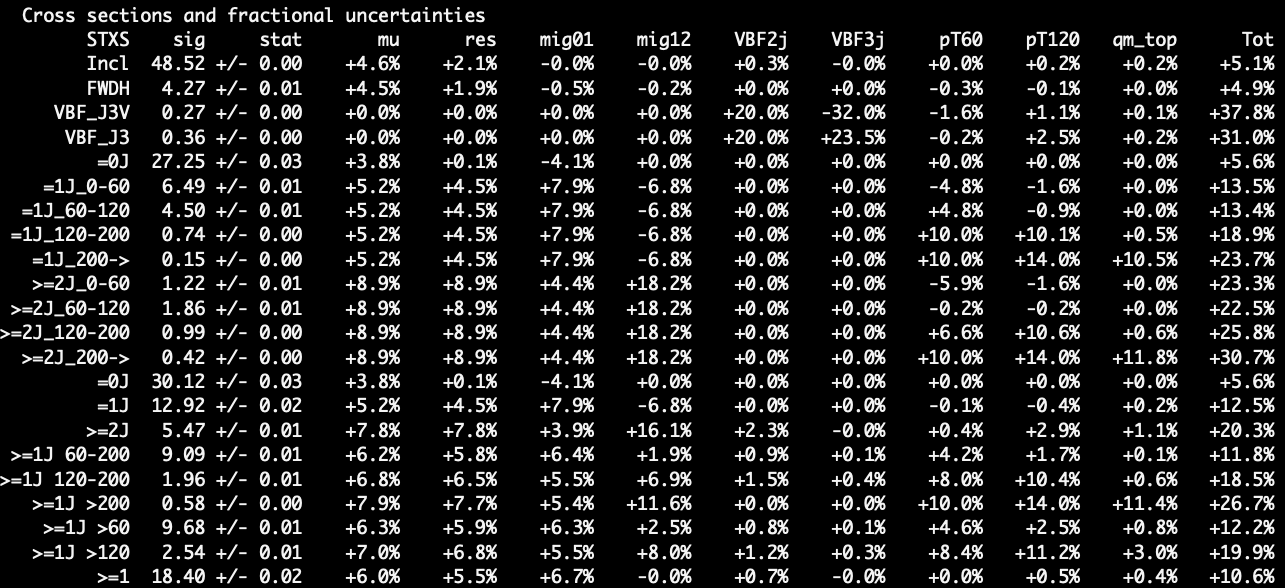
\includegraphics[width=0.9\textwidth]{Figures/Systematics/ggH_unc.png}
%		\caption{Summary of the theory systematic uncertainties of the ggH production modes in $\Hllll$ measurements for the stage 1.1 analysis
%		\label{fig:ggH_sys}}
%	\end{center}
%\end{figure}
%
%
%\begin{table}[!htb]
%\begin{center}
%\small
%\caption{Summary of the theory systematic uncertainties of the non-ggH production modes in $\Hllll$ measurements for the stage 1.1 analysis
%\label{tab:SystOverviewTheo}
%}
%\begin{tabular}{|c|c|c|c|c|}
%\hline %---------------------------------------------------------
%%\vspace{-0.4cm} & \\
%& QCD scale $\mu$R & QCD scale $\mu$F & PDF set  & PDF AlphaS \\ 
%\hline %---------------------------------------------------------
%VBF\_2j\_mjj\_350\_700\_2j&  $0.9$& $1.0$& $3.7$& $0.6$\\ 
%VBF\_2j\_mjj\_GT700\_2j&     $0.4$& $1.0$& $5.6$& $0.5$\\ 
%VBF\_2j\_mjj\_GT350\_3j&     $0.1$& $0.1$& $5.6$& $0.6$\\ 
%VBF\_Rest& 		     $0.5$& $0.7$& $4.4$& $0.7$\\ 
%VBF\_GT200&		     $0.7$& $1.0$& $6.7$& $0.4$\\ 
%VH\_Had&	             $4.8$& $5.2$& $3.9$& $0.7$\\ 
%VH\_Lep\_0\_150&	     $3.6$& $1.6$& $3.7$& $0.8$\\ 
%VH\_Lep\_GT150&		     $3.7$& $4.9$& $3.9$& $0.9$\\ 
%ttH&		     	     $4.3$& $2.8$& $3.2$& $1.5$\\ 
%\hline %---------------------------------------------------------
%\end{tabular}
%\normalsize
%\end{center}
%\end{table}
%
%\begin{table}[!htb]
%\begin{center}
%\small
%
%\caption{Summary of the systematic uncertainties in the $\Hllll$ measurements on the categorization migration
%
%\label{tab:SystOverviewTheo_cat}
%}
%\begin{tabular}{|c|c|} %|c|c|}
%\hline %---------------------------------------------------------
%\hline %---------------------------------------------------------
%\multicolumn{2}{|c|}{\textbf{Summary of  the systematic uncertainties on the categorization migration}} \\
%\hline %---------------------------------------------------------
%\hline %---------------------------------------------------------
%%\vspace{-0.4cm} & \\
%% & 2016 & 2017 & 2018 \\
%%\hline %--------------------------------------------- ------------
%QCD scale $\mu$R(${\rm gg}$) & 0.1--6 \%  \\% & XX \% & XX \% \\
%\vspace{-0.4cm} & \\%& XX \% & XX \% \\
%QCD scale $\mu$F(${\rm gg}$) & 0.1--6 \% \\%& XX \% & XX \% \\
%\vspace{-0.4cm} & \\%& XX \% & XX \% \\
%PDF set (${\rm gg}$) & $$ 0.1--2 \% \\%& XX \% & XX \%  \\
%\vspace{-0.4cm} & \\
%PDF AlphaS(${\rm gg}$) & $$ 0.1--2 \% \\%& XX \% & XX \%  \\
%\vspace{-0.4cm} & \\
%QCD scale $\mu$R(${\rm VBF,\rm WH, \rm ZH}$) & 0.1--12 \% \\%& XX \% & XX \%  \\
%\vspace{-0.4cm} & \\
%QCD scale $\mu$F(${\rm VBF,\rm WH, \rm ZH}$) & 0.1--6 \% \\%& XX \% & XX \%  \\
%\vspace{-0.4cm} & \\
%PDF set (${\rm VBF,\rm WH, \rm ZH}$) & $$ 0.1--5 \% \\%& XX \% & XX \%  \\
%\vspace{-0.4cm} & \\
%PDF AlphaS(${\rm VBF,\rm WH, \rm ZH}$) & $$ 0.1--2 \% \\%& XX \% & XX \%  \\
%\vspace{-0.4cm} & \\
%QCD scale $\mu$R(${\rm ttH}$) & 0.1--8 \% \\ % & XX \% & XX \% \\
%\vspace{-0.4cm} & \\
%QCD scale $\mu$F(${\rm ttH}$) & 0.1--3 \% \\%& XX \% & XX \% \\
%\vspace{-0.4cm} & \\
%PDF set (${\rm ttH}$) & $$ 0.2--1 \% \\%& XX \% & XX \% \\
%\vspace{-0.4cm} & \\
%PDF AlphaS(${\rm ttH}$) & $$ 0.1--0.7 \% \\%& XX \% & XX \% \\
%\vspace{-0.4cm} & \\
%JES & $$ 1--200 \% \\%& XX \% & XX \% \\
%\vspace{-0.4cm} & \\
%JER & $$ 1--55 \% \\%& XX \% & XX \% \\
%\vspace{-0.4cm} & \\
%Btag & $$ 1--22 \% \\%& XX \% & XX \% \\
%\hline %--------------------------------------------------------
%\end{tabular}
%\normalsize
%\end{center}
%\end{table}
%
%\vspace{-0.4cm} & \\
%\hline %---------------------------------------------------------
%\hline %---------------------------------------------------------
%\end{tabular}
%\normalsize
%\end{center}
%\end{table}

%\begin{figure}[!htb]
%\vspace*{0.3cm}
%\begin{center}
%\includegraphics[width=0.3\textwidth]{Figures/Systematics/HtoZZ4mu_JJVBFTagged_FinalTemplates_ggZZ_Nominal.pdf}
%\includegraphics[width=0.3\textwidth]{Figures/Systematics/HtoZZ4mu_JJVBFTagged_FinalTemplates_ggZZ_CMS_scale_j_13TeV_2017Up.pdf}
%\includegraphics[width=0.3\textwidth]{Figures/Systematics/HtoZZ4mu_JJVBFTagged_FinalTemplates_ggZZ_CMS_eff_mUp.pdf} \\
%\includegraphics[width=0.3\textwidth]{Figures/Systematics/HtoZZ4mu_JJVBFTagged_FinalTemplates_VBF_Nominal.pdf}
%\includegraphics[width=0.3\textwidth]{Figures/Systematics/HtoZZ4mu_JJVBFTagged_FinalTemplates_VBF_CMS_tune_pythiaUp.pdf}
%\includegraphics[width=0.3\textwidth]{Figures/Systematics/HtoZZ4mu_JJVBFTagged_FinalTemplates_VBF_CMS_eff_mUp.pdf} \\
%\includegraphics[width=0.3\textwidth]{Figures/Systematics/HtoZZ4mu_JJVBFTagged_FinalTemplates_WH_Nominal.pdf}
%\includegraphics[width=0.3\textwidth]{Figures/Systematics/HtoZZ4mu_JJVBFTagged_FinalTemplates_WH_CMS_tune_pythiaUp.pdf}
%\includegraphics[width=0.3\textwidth]{Figures/Systematics/HtoZZ4mu_JJVBFTagged_FinalTemplates_WH_CMS_eff_mUp.pdf} \\
%
%\caption{
%Conditional distribution of $\DbkgVBFdec$ in the VBF-2 jets tagged category for the 4mu channel,  as a function of $m_{4\ell}$, for ggH (top row), VBF (middle row) and WH (bottom row). Templates are shown for the nominal configuration (left column), the dominant uncertainties (jet energy scale for ggH, pythia tune for VBF and WH) in the middle column and a sub-dominant one (uncertainties on leptons momentum) in the right column.
%\label{fig:alt_template}}
%\end{center}
%\end{figure}

%Theoretical systematics on scale and category migrations due to QCD scale in gluon fusion are calculated using the so called WG1 uncertainty scheme. There are 9 uncertainties in total, 2 of which correspond to scale change (THU\_ggH\_Mu and THU\_ggH\_Res) and 7 others to category migrations. 

\subsection{Systematic uncertainties treatment when combining the data sets}

In this Section we describe how different systematic uncertainties are treated when combining the data sets. The theoretical uncertainties are correlated. All the experimental systematics are treated indepandently.

%\subsection{Impact plots}
%
%The Fig.~\ref{fig:impact}.shows the impact of the difference sources of uncertainties on the inclusive signal strength measurement. The largest contributions come from the lepton efficiency uncertainty, the luminosity and theoretical uncertainties associated to gluon fusion production mode. Uncertainties related to jet have a larger impact in categories targeting, for instance, VBF production mode.
%%They give largest contribution to the overall systematics from the theoretical part while all other theoretical uncertainties mentioned here do not have a significant impact as it can be seen on the Fig.~\ref{fig:impact}.
%
%\begin{figure}[!htb]
%\vspace*{0.3cm}
%\begin{center}
%\subfigure[]{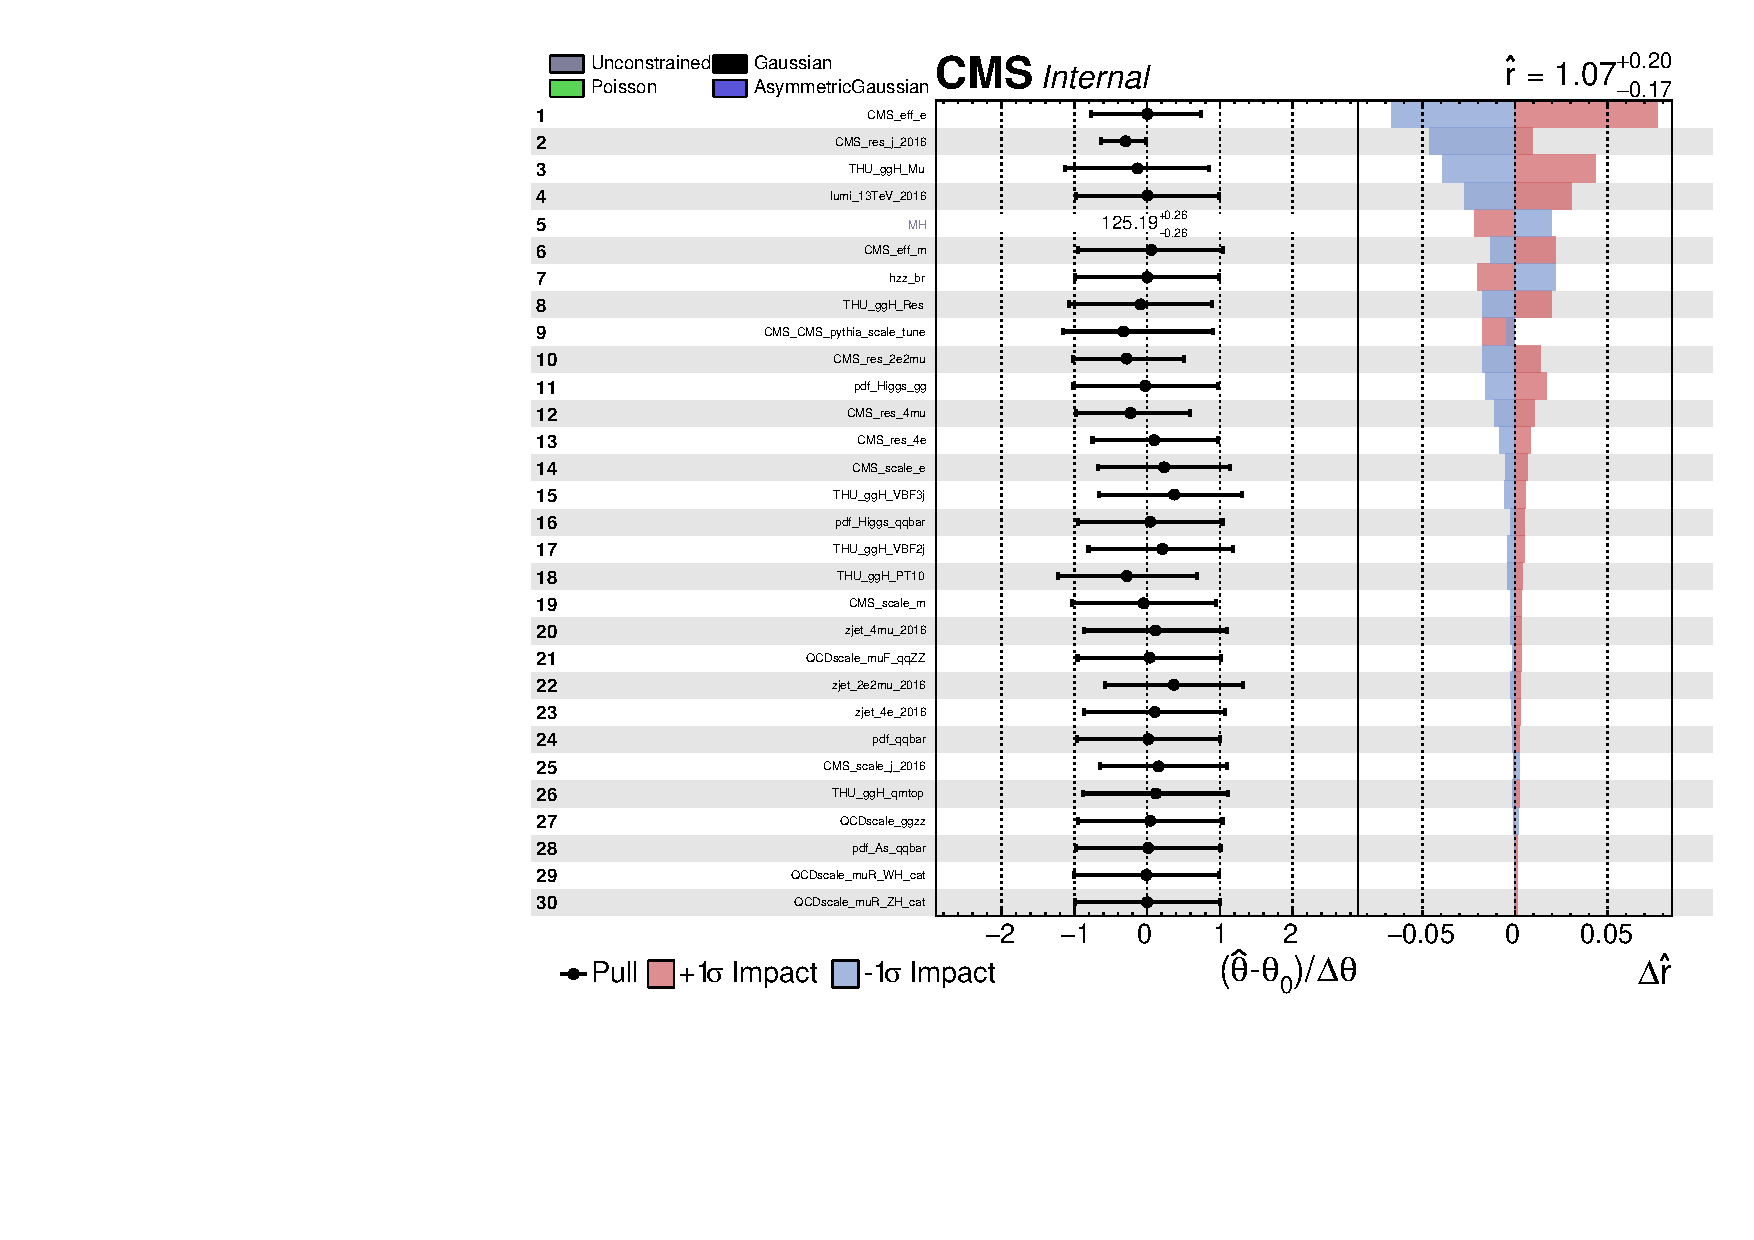
\includegraphics[width=0.45\textwidth]{Figures/Systematics/impacts_16.pdf}} 
%\subfigure[]{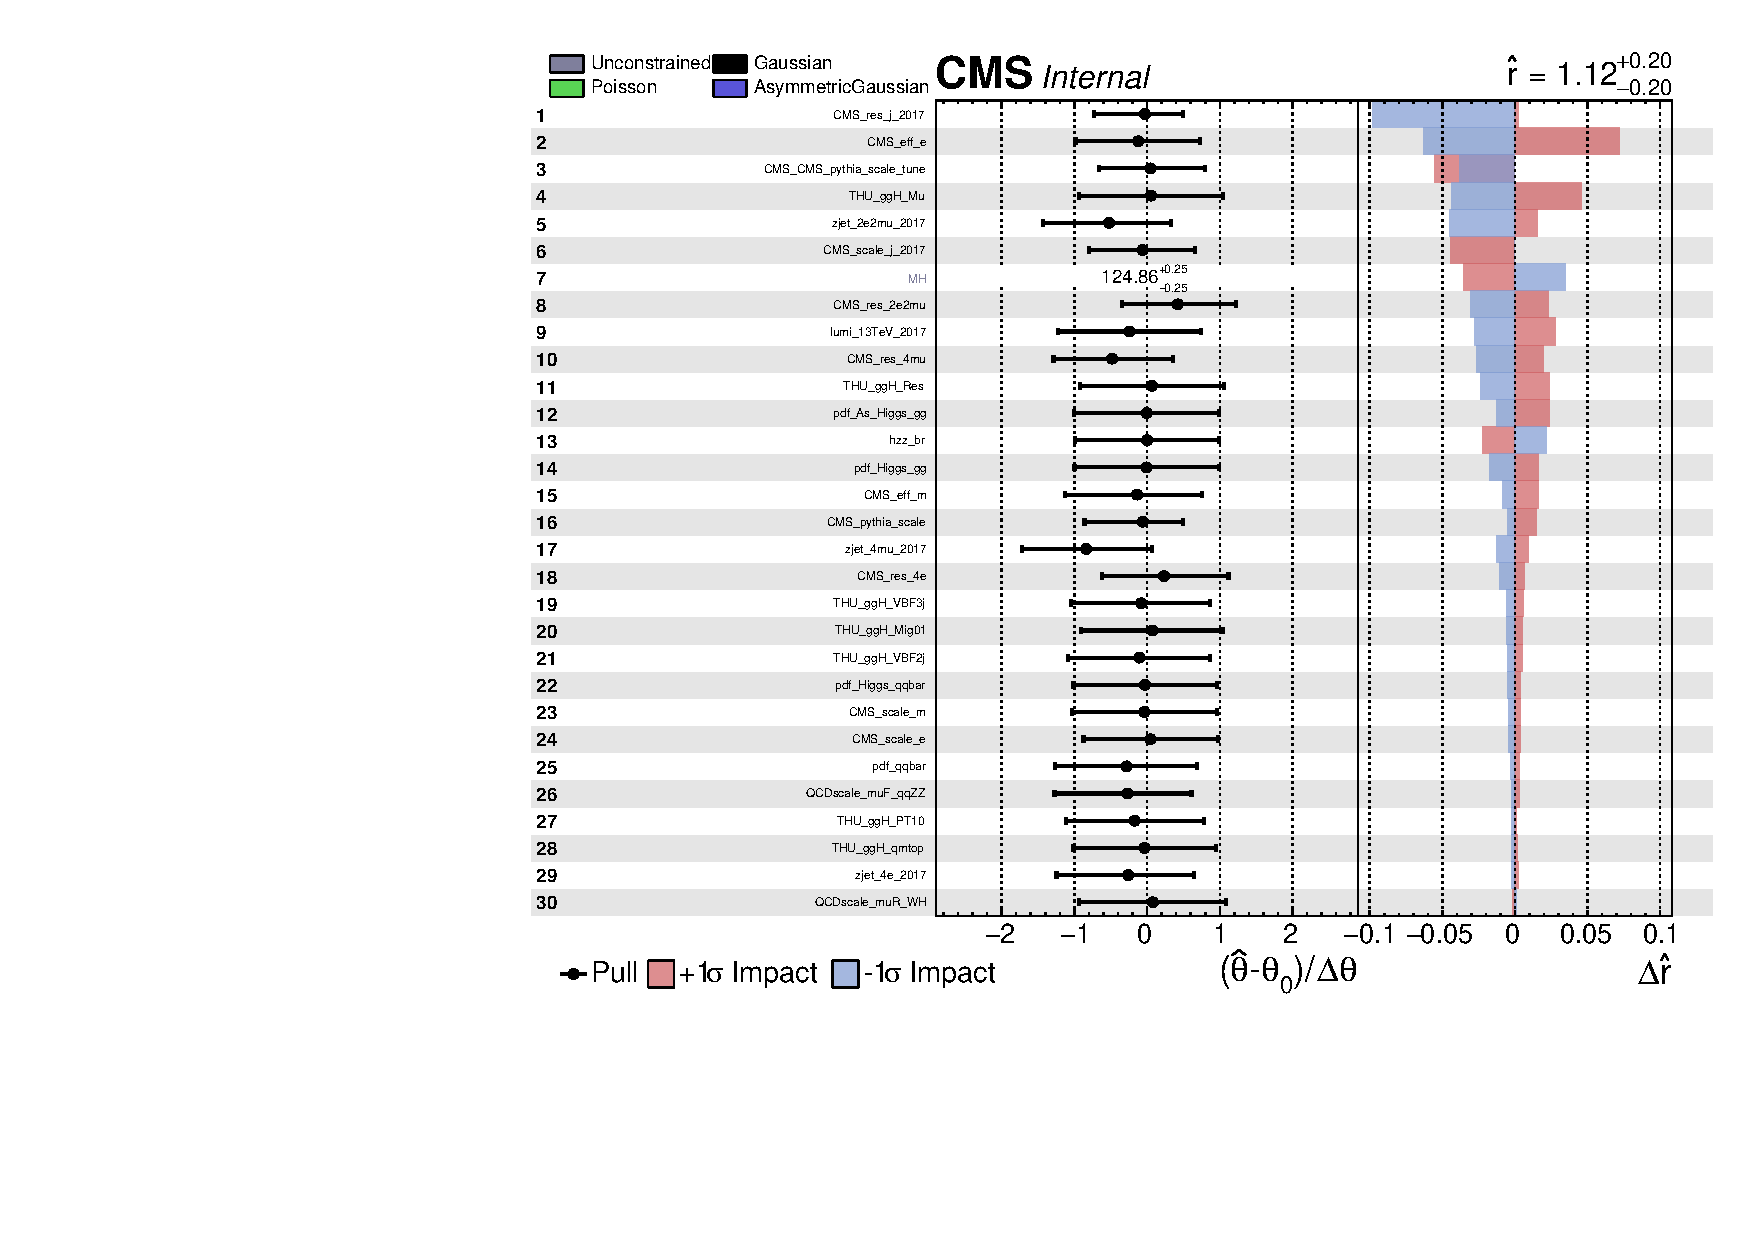
\includegraphics[width=0.45\textwidth]{Figures/Systematics/impacts_17.pdf}} \\
%\subfigure[]{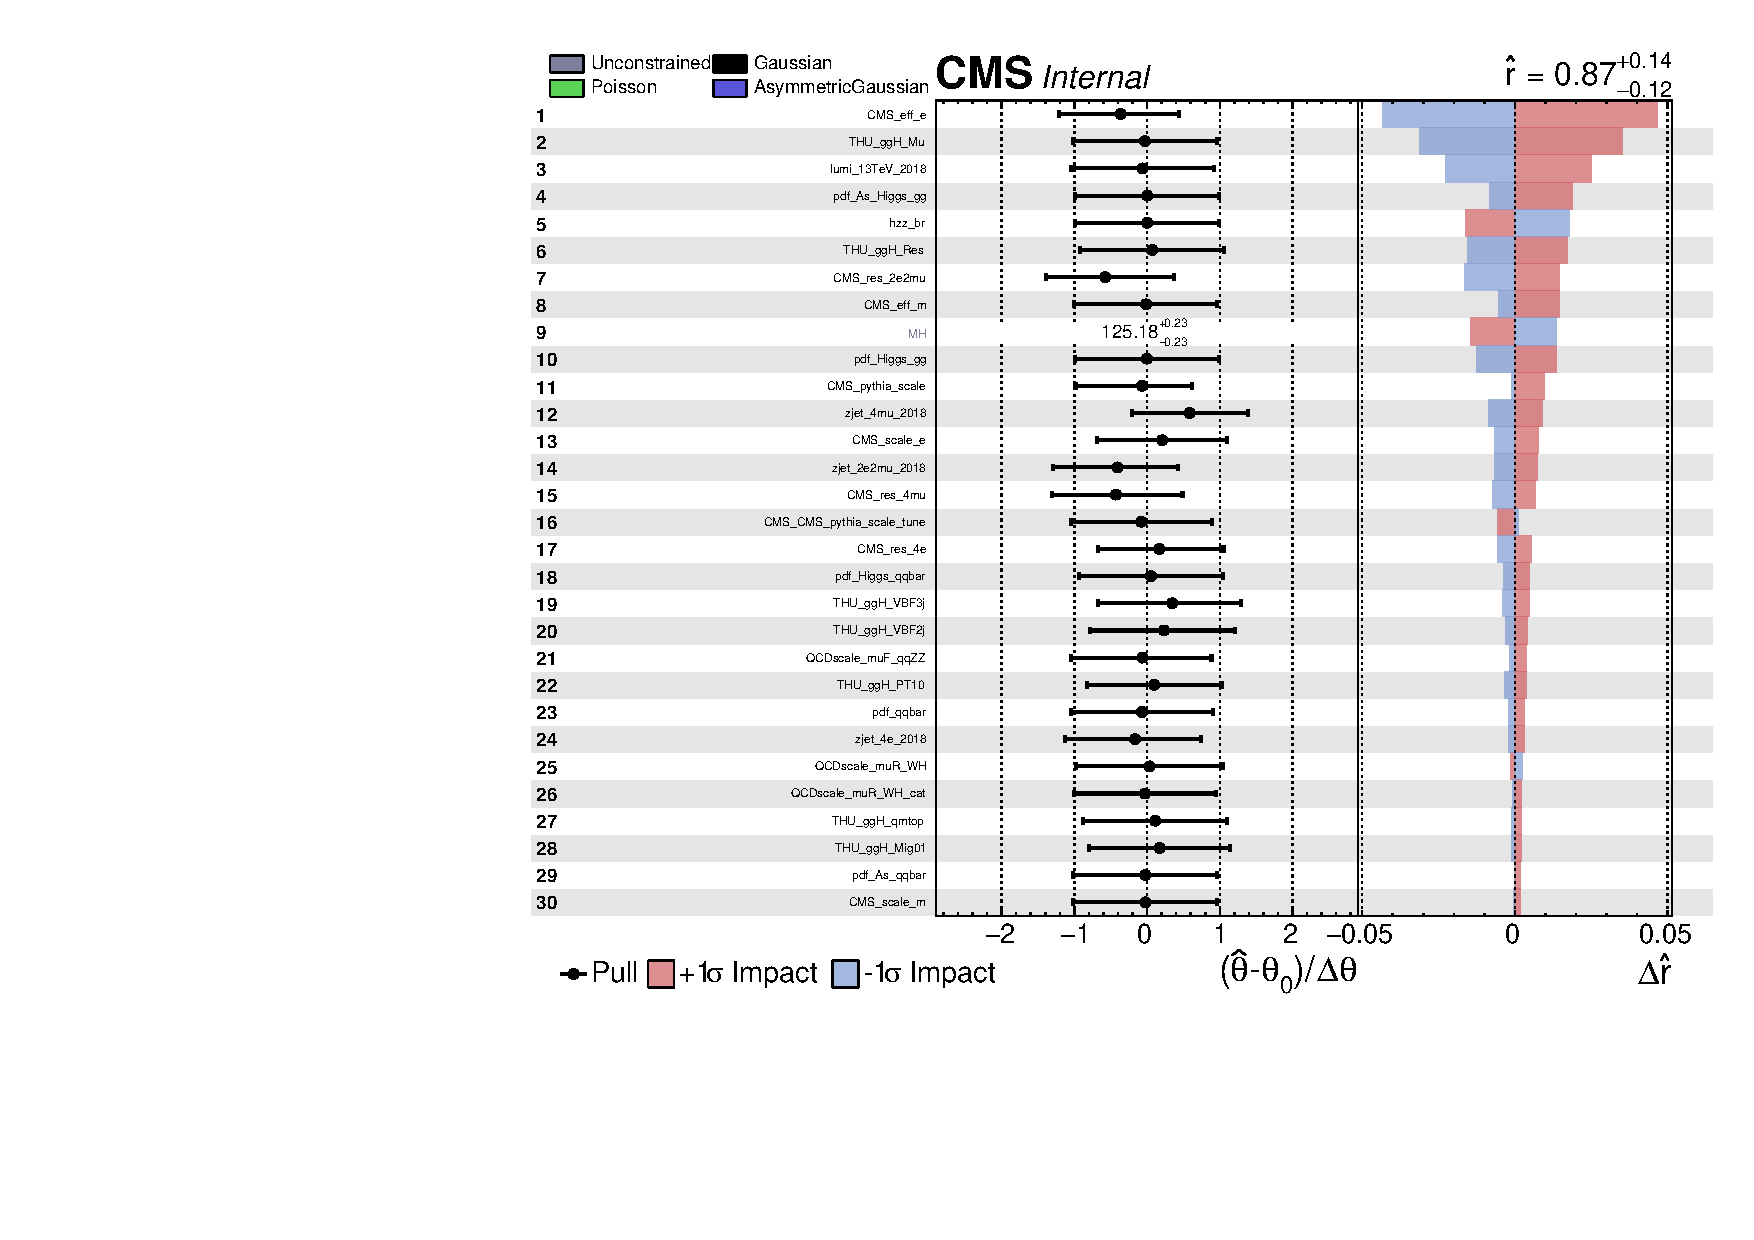
\includegraphics[width=0.45\textwidth]{Figures/Systematics/impacts_18.pdf}} 
%\subfigure[]{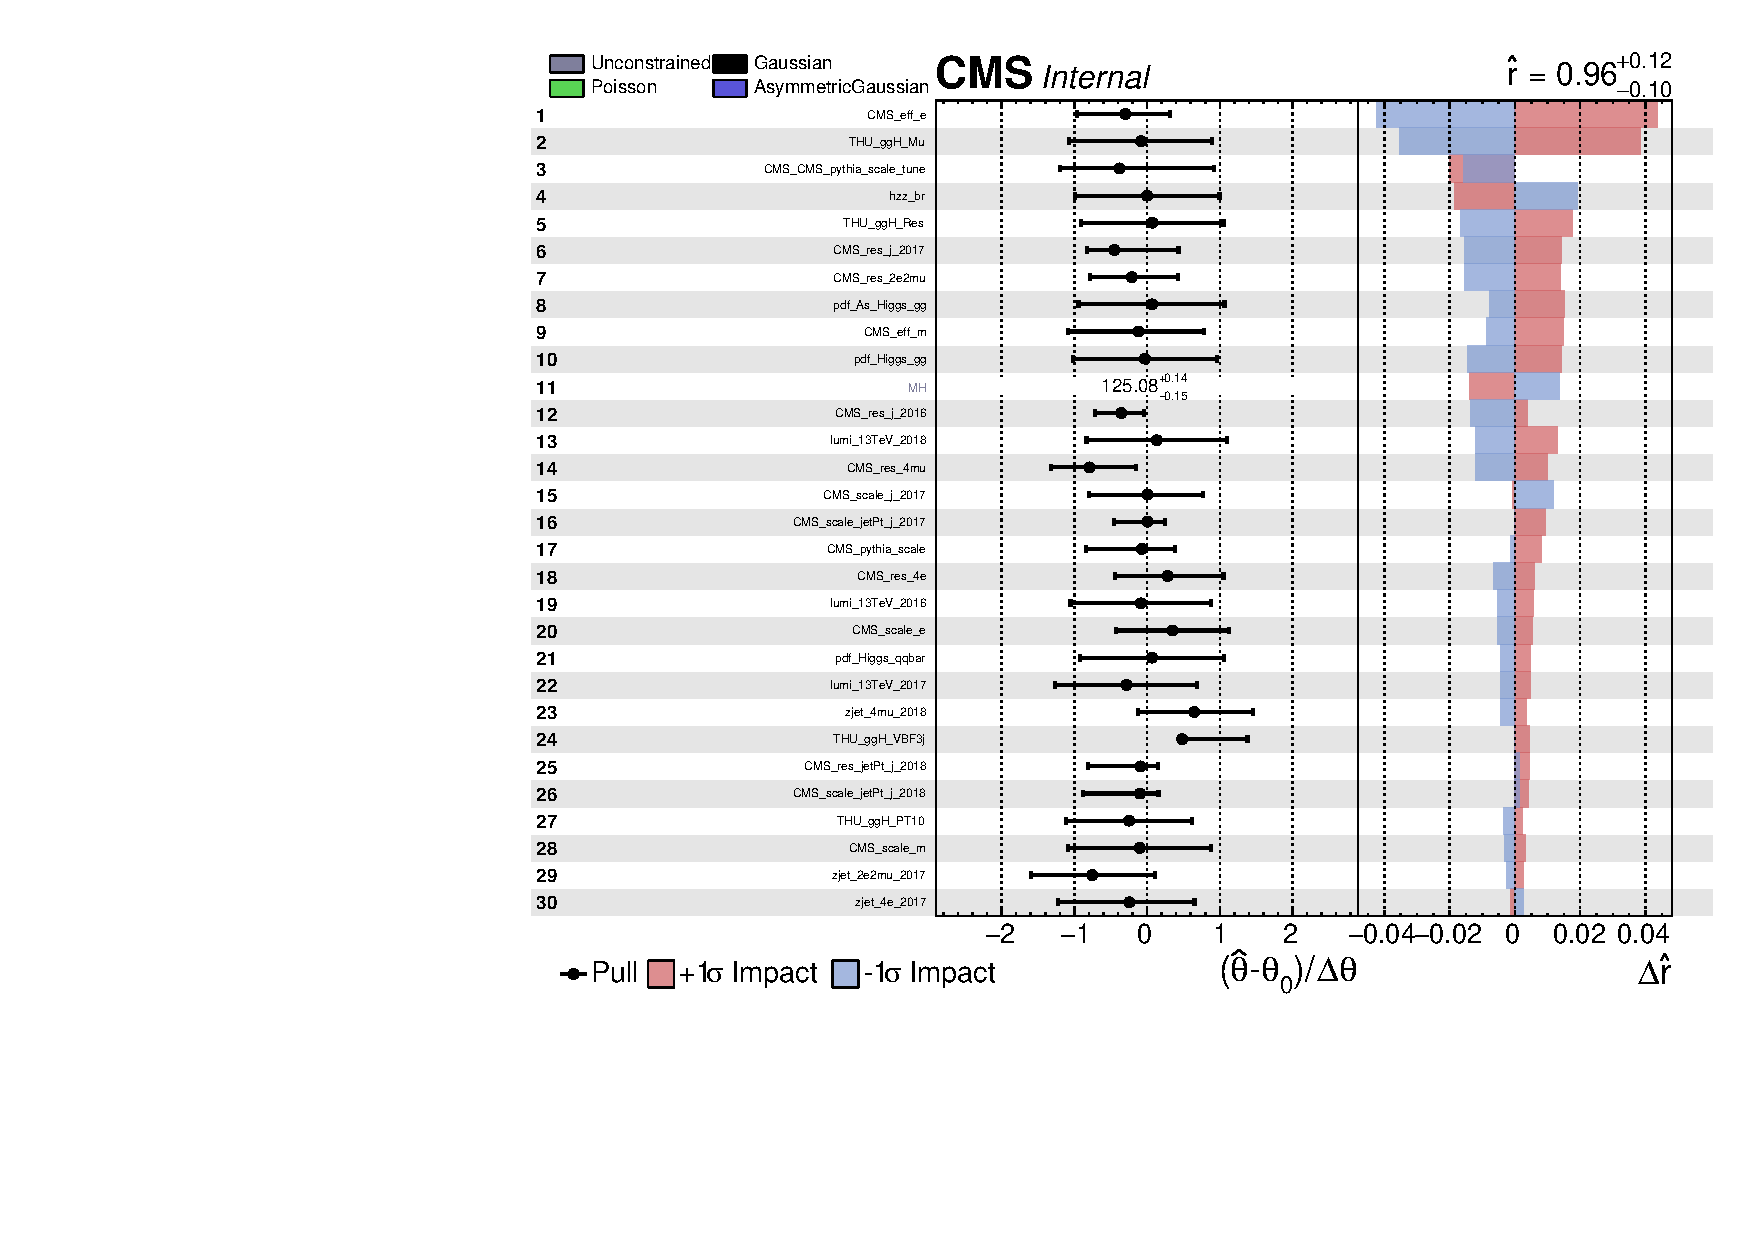
\includegraphics[width=0.45\textwidth]{Figures/Systematics/impacts_RunII.pdf}}  
%%\includegraphics[page=2, width=0.7\textwidth]{Figures/Systematics/impacts_new.pdf}\\
%\caption{
%Pulls for 2016 data (top left), 2017 data (top right), 2018 data (bottom left) and all data combined (bottom right).
%\label{fig:impact}}
%\end{center}
%\end{figure}
